\documentclass{article}

\usepackage[margin=1in]{geometry}
\usepackage{amsmath,amsthm,amssymb}
\usepackage{bbm,enumerate,mathtools}
\usepackage[hidelinks]{hyperref}
\usepackage{tikz}
\usetikzlibrary{matrix, arrows}

\newenvironment{problem}[2][Problem]{\begin{trivlist}
\item[\hskip \labelsep {\bfseries #1}\hskip \labelsep {\bfseries #2.}]}{\end{trivlist}}
\newenvironment{solution}[1][Solution.]{\begin{trivlist}
\item[\hskip \labelsep {\bfseries #1}]}{\end{trivlist}}
\newenvironment{problempart}[1]{\begin{trivlist}\item[\textbf{Part #1.}]}{\end{trivlist}}
\newcommand{\set}[1]{\{ #1 \}}
\newcommand{\ang}[1]{\langle #1 \rangle}
\begin{document}

\title{Combinatorics: Homework 9}
\author{Peter Kagey}

\maketitle

% -----------------------------------------------------
% First problem
% -----------------------------------------------------
\begin{problem}{34} $[2]$ \\
  Find all nonisomorphic posets P such that \[
    F(J(P), x) = (1 + x)(1 + x^2)(1 + x + x^2)
  \]
\end{problem}

\begin{solution}
  $F(J(P), x) = 1 + 2x + 3x^2 + 3x^3 + 2x^4 + x^5$, so $J(P)$ has rank $5$ so
  $P$ has five elements, call them $\{1,2,3,4,5\}$

  Since the coefficient of $x$ in $F(J(P), x)$ is $2$ there must be
  exactly two minimal elements in $P$. Name these $1$ and $2$. The
  remaining three elements of the poset are not minimal, so they must be greater
  than $1$ or $2$ or both.
  Without loss of generality, say that $1 \lessdot 3$.
  \\~\\
  \textbf{Case 1.} Assume $1 \lessdot 3$ and $2 \lessdot 3$.\\
  Thus the Hasse diagram looks like this (where the orders on 4 and 5 still
  need to be drawn): \[
    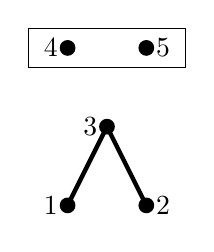
\begin{tikzpicture}
      \fill (0,0) circle (0.1) node[left] {1};
      \fill (1/2,1) circle (0.1) node[left] {3};
      \draw[ultra thick] (0,0)--(1/2,1);

      \fill (1,0) circle (0.1) node[right] {2};
      \draw[ultra thick] (1,0)--(1/2,1);

      \draw (-1/2,7/4) rectangle (3/2, 9/4);
      \fill (0,2) circle (0.1) node[left] {4};
      \fill (1,2) circle (0.1) node[right] {5};
    \end{tikzpicture}
  \]
  This diagram (ignoring $4$ and $5$) has
  two one-element ideals (namely $\set 1$ and $\set 2$),
  but only one two-element ideal (namely $\set{1,2}$). There are two ways
  (without loss of generalization) to
  put orders on $4$ and $5$ that add two two-element ideals but no one-element
  ideals \[
    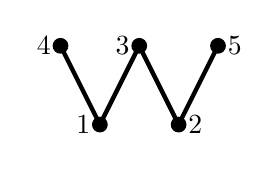
\begin{tikzpicture}
      \fill (0,0) circle (0.1) node[left] {1};
      \fill (1,0) circle (0.1) node[right] {2};
      \fill (1/2,1) circle (0.1) node[left] {3};
      \fill (-1/2,1) circle (0.1) node[left] {4};
      \fill (3/2,1) circle (0.1) node[right] {5};

      \draw[ultra thick] (-1/2,1)--(0,0)--(1/2,1)--(1,0)--(3/2,1);
    \end{tikzpicture}
    \hspace{1cm}\text{and}\hspace{1cm}
    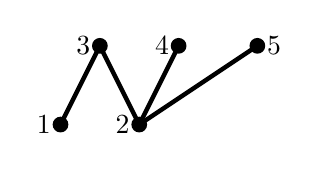
\begin{tikzpicture}
      \fill (0,0) circle (0.1) node[left] {1};
      \fill (1,0) circle (0.1) node[left] {2};
      \fill (1/2,1) circle (0.1) node[left] {3};
      \fill (3/2,1) circle (0.1) node[left] {4};
      \fill (5/2,1) circle (0.1) node[right] {5};

      \draw[ultra thick] (0,0)--(1/2,1)--(1,0)--(3/2,1);
      \draw[ultra thick] (1,0)--(5/2,1);
    \end{tikzpicture}
  \]

  The poset $P_\text{right}$ on the right has three $4$-element ideals,
  $\ang{3, 4} = \set{1,2,3,4}$,
  $\ang{3, 5} = \set{1,2,3,5}$, and
  $\ang{4, 5} = \set{1,2,4,5}$,
  so the coefficient of $x^4$ in $F(J(P_\text{right}),x)$ is $3$ not $2$ as
  desired.

  The poset $P_\text{left}$ on the left has four $3$-element ideals:
  $\ang{1,4}$, $\ang{1,5}$, $\ang 3$, and $\ang{4, 5}$,
  so the coefficient of $x^3$ in $F(J(P_\text{left}),x)$ is $4$ not $3$ as
  desired.
  Thus there are no posets such that $1 \lessdot 3$ with the desired
  rank generating function.
  \\~\\
  \textbf{Case 2.} Assume $1 \lessdot 3$ and $2 \not\leq 3$.\\
  Since there are no posets from Case 1 that work, any
  valid posets must be from case two.
  There is no element $3$ such that $1 \lessdot 3$ and $2 \lessdot 3$, so
  the graph has two connected components $P_1 + P_2$. Assume without loss of
  generality that $P_1$ (which contains $1$ and $3$) has more elements than
  $P_2$, that is so $P_1$ has either $3$ or $4$ elements, and $P_2$ has $2$ or
  $1$ element respectively.
  If $P_2 = \set 2$ has just one element, then $1$ must be covered by one, two, or three
  elements.
  \begin{enumerate}
    \item If $1$ is covered only by $3$, then the poset has only two $2$-element
    ideals, namely $\ang{1, 2}$ and $\ang 3$.
    \item  If $1$ is covered by two elements (call these $3$ and $4$ without loss of
    generality) then in order to avoid having too many $1$, $2$, or $3$-element
    ideals, $5$ must cover both $3$ and $4$.
    \item If $1$ is covered by $3, 4,$ and $5$, then the poset has only four $2$-element
    ideals, namely $\ang{1, 2}, \ang 3, \ang 4,$ and $\ang 5$.
  \end{enumerate}
  Thus if $P_2 = \set 2$, then the only partial order that will work is \[
    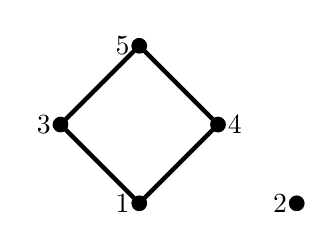
\begin{tikzpicture}
      \fill (0,0) circle (0.1) node[left] {1};
      \fill (2,0) circle (0.1) node[left] {2};
      \fill (-1,1) circle (0.1) node[left] {3};
      \fill (1,1) circle (0.1) node[right] {4};
      \fill (0,2) circle (0.1) node[left] {5};
      \draw[ultra thick] (0,0)--(-1,1)--(0,2)--(1,1)--cycle;
    \end{tikzpicture}
  \]
  On the other hand, if $P_2 = \set{2,4}$ with $2 \lessdot 4$, then we have two
  cases \begin{enumerate}
    \item If $1$ is covered only by $3$ (and thus $5 \lessdot 3$), then this satisfies the rank generating
    function.
    \item If $1$ is covered by two element, $3$ and $5$ and $5$, then the poset
    has four $2$-element ideals, namely $\ang{1, 2}, \ang 3, \ang 4,$ and $\ang 5$.
  \end{enumerate}
  So the poset $P = [3] + [2]$ also works: \[
    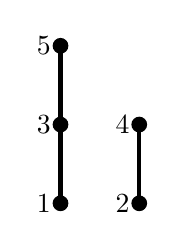
\begin{tikzpicture}
      \fill (0,0) circle (0.1) node[left] {1};
      \fill (0,1) circle (0.1) node[left] {3};
      \fill (1,0) circle (0.1) node[left] {2};
      \fill (1,1) circle (0.1) node[left] {4};
      \fill (0,2) circle (0.1) node[left] {5};
      \draw[ultra thick] (0,0)--(0,2);
      \draw[ultra thick] (1,0)--(1,1);
    \end{tikzpicture}
  \]
  % In the first case, $J([2] + [3]) = [3] \times [4]$, and $F([3] \times [4], x)$
  % matches the desired rank generating function.
  % \\
  % In the second case, $J(P)$ has only two ideals with three elements, so the
  % coefficient of $x^3$ is $2$, not $3$ as desired.
  % \\
  % In the third case, $J(P)$, has four ideals of with two elements, so the
  % coefficient of $x^2$ is $4$, not $3$ as desired.
  % \\~\\
  % Thus the only choice that works is $P = [2] + [3]$.
\end{solution}
\pagebreak
% -----------------------------------------------------
% Second problem
% -----------------------------------------------------
\begin{problem}{46 a} $[2]$ \\
  Let $f(n)$ be the number of sublattices of rank $n$ of the boolean algebra
  $B_n$. Show that $f(n)$ is also the number of partial orders $P$ on $[n]$.
\end{problem}

\begin{solution} \text{} \\
  Since $B_n$ is a distributive lattice, all rank $n$ sublattices of $B_n$ must
  also be distributive lattices. Thus each sublattice of $L \subset B_n$ can be
  written as $L \cong J(P)$ for some poset $P$, where $P$ is isomorphic to the
  set of join irreducibles of $L$. By proposition 3.4.5, since $L$ has rank $n$,
  $P$ must have $n$ elements. So every distributive lattices of rank $n$ gives
  a partial ordering of $[n]$.
  \\~\\
  This a bijection, because given some poset $P$, we can recover $L$ via $J$
  (namely, $L \cong J(P)$). Each distinct $P$ gives a distinct rank $n$
  sublattice of $B_n$ because
  (1) $J(P)$ is a distributive lattice,
  (2) $J(P)$ contains the ideal $[n]$,
  (and no larger ideal) and,
  (3) $J(P)$ includes the ideal $\emptyset$.
  % Let $\phi$ be a map which sends a poset $P$ (with underlying set $[n]$) to
  % $J(P) \subset B_n$.
  % Since $B_n$ is a finite distributive lattice, and every sublattice of a
  % finite distributive lattice is a finite distributive lattice, we can
  % take the set of join irreducibles of any rank $n$ sublattice, and this will
  % be isomorphic to a poset on $[n]$.
\end{solution}
\pagebreak
% -----------------------------------------------------
% Third problem
% -----------------------------------------------------
\begin{problem}{53} $[2]$ \\
  Let $P$ be a finite $n$-element poset. Simplify the two sums \[
    f(P) = \sum_{I \subset J(P)} e(I)e(\overline I),
  \] \[
    g(P) = \sum_{I \subset J(P)} \binom{n}{\#I} e(I)e(\overline I),
  \] where $\overline I$ denotes the complement $P - I$ of the order ideal $I$.
\end{problem}

\begin{proof}
  The pre-image $\sigma^{-1}([j])$ of a linear extension $\sigma$ is a
  $j$-element ideal. In particular, every ideal can be written as
  $\sigma^{-1}([j])$ for some linear extension.
  Therefore each linear extension has $n+1$ associated ideals, namely,
  $\sigma^{-1}([k])$ for $k \in [n]$ along with $\sigma^{-1}(\emptyset)$.
  Therefore since $P - \sigma^{-1}([j])$ has the relative order of a linear
  extension, the sum given by $f$ overcounts each linear extension of $P$
  exactly $n + 1$ times, so
  \[
    f(P) = (n + 1)e(P).
  \]
\end{proof}
\pagebreak
% -----------------------------------------------------
% Fourth problem
% -----------------------------------------------------
\begin{problem}{57} ~
  \begin{enumerate}[a.]
    \item $[2]$ Let $P$ be an $n$-element poset. If $t \in P$, then set
    $\lambda_t = \#\{s \in P : s \leq t\}$.
    Show that \[
      e(P) \geq \frac{n!}{ \prod_{t \in P} \lambda_t}.
    \]
    \item $[2+]$ Show that the equality holds if and only if every component of $P$ is
    a rooted tree.
  \end{enumerate}
\end{problem}

\begin{proof}
  \begin{enumerate}[a.]
    \item By induction, the base case is clear. When $n=1$, there is only
    one poset with one linear extension. \[
      e([1]) = \frac{1!}{\lambda_{1}} \geq 1.
    \]
    Thus given some poset $P$, we can take the subposet $P - m$ (where $m$ is
    any maximal element in $P$) which is a disjoint union of posets
    $P_1 + P_2 + \hdots + P_k$ with $n_1, n_2, \hdots, n_k$ elements respectively.
    There are $n - \lambda_m + 1$ choices of labels for $m$. After choosing one,
    $n_i$ labels for each $P_i$ can be chosen, and each can be
    permuted in $e(P_i)$ ways, so \begin{align*}
      e(P) &= (n - \lambda_m + 1)\binom{n - 1}{n_1, n_2, \hdots, n_k}e(P_1)e(P_2)\hdots e(P_k) \\
      &\geq (n - \lambda_m + 1)
      \frac{(n - 1)!}{n_1! n_2! \hdots n_k!} \cdot
      \frac{n_1!}{\prod_{t \in P_1} \lambda_t}\cdot
      \frac{n_2!}{\prod_{t \in P_2} \lambda_t}
      \cdots
      \frac{n_k!}{\prod_{t \in P_k} \lambda_t} \\
      &= (n - \lambda_m + 1)\frac{(n-1)!}{\prod_{t\in P- m} \lambda t}
    \end{align*}
    Since $\lambda m$ must take on values in $[n]$,
    $\lambda_m(n - \lambda_m + 1)$ is concave down with respect to $\lambda_m$
    and so has minima at $\lambda_m = 1$ and $\lambda_m = n$, in particular
    $n - \lambda_m + 1 \geq n/\lambda_m$ so substituting this into the
    inequality above gives \[
    e(P) \geq \frac{n}{\lambda_m}\cdot \frac{(n-1)!}{\prod_{t\in P- m} \lambda t}
    = \frac{n!}{\prod_{t\in P} \lambda t},
    \] as desired.
    %
    \item $(\Longrightarrow)$
    Assume that the equality holds. This means that in the above argument, for
    each maximal element $m$, $\lambda_m = 1$ or $\lambda_m = n$.
    If $\lambda_m = 1$, then the component containing $m$ is the singleton poset
    and thus is a rooted tree. If $\lambda_m = n$, then $m$ must be the unique
    maximal element of its component, $m = \hat 1_{P_i}$.
    \\
    By the above argument, this can be repeated inductively; that is, after
    removing any maximal element, the new maximal elements have the same
    property. Therefore $P_i$ is a rooted tree for all components $P_i$ of $P$.
    \\~\\
    $(\Longleftarrow)$
    \\
    By induction, the base case is clear. When $n=1$, there is only
    one poset (which is a rooted tree) with one linear extension. \[
      e([1]) = \frac{1!}{\lambda_{1}} = 1.
    \]
    Thus given some rooted tree $P$, we can take the subposet $P - \hat 1$, which
    is a disjoint union of rooted trees
    $P_1 + P_2 + \hdots + P_k$ with $n_1, n_2, \hdots, n_k$ elements respectively.
    Since $P$ has a unique maximum, it must be labeled with $n$, then we can
    then choose which letters go in each sub-tree (using a multinomial
    coefficient), and then there are $e(P_i)$ ways to order the $n_i$ labels
    for each $P_i$. Therefore \begin{align*}
        e(P) &= \binom{n - 1}{n_1, n_2, \hdots, n_k}e(P_1)e(P_2)\hdots e(P_k)
        \\
        &= \binom{n - 1}{n_1, n_2, \hdots, n_k}
        \frac{n_1!}{\prod_{t \in P_1} \lambda_t}
        \frac{n_2!}{\prod_{t \in P_2} \lambda_t}
        \hdots
        \frac{n_k!}{\prod_{t \in P_k} \lambda_t}
        \\
        &= \left(\frac{(n - 1)!}{n_1! n_2! \hdots n_k!}\right)
        \frac{n_1!n_2!\hdots n_k!}{\prod_{t \in P - \hat 1} \lambda_t}
        \\
        &= \frac{(n-1)!}{\prod_{t \in P - \hat 1} \lambda_t}
    \end{align*}
    Since all $n$ elements of $P$ are less than or equal to $\hat 1$,
    $\lambda_{\hat 1} = n$, \[
      n\prod_{t \in P - \hat 1} \lambda_t = \prod_{t \in P} \lambda_t
    \] and thus \[
      e(P) = \frac{n(n-1)!}{n\prod_{t \in P - \hat 1} \lambda_t} = \frac{n!}{\prod_{t \in P} \lambda_t}
    \] as desired.
  \end{enumerate}
\end{proof}
\end{document}
